\documentclass[../../main.tex]{subfiles}
\cite{pfyfferhistorischeslexikon}
\cite{patrizischeortehistorischeslexikon}
\cite{patriziathistorischeslexikon}
\cite{familiepfyfferwikipedia}
\cite{grandhotelkulturgut}
\paragraph{}
\begin{figure}[h]
    \centering
    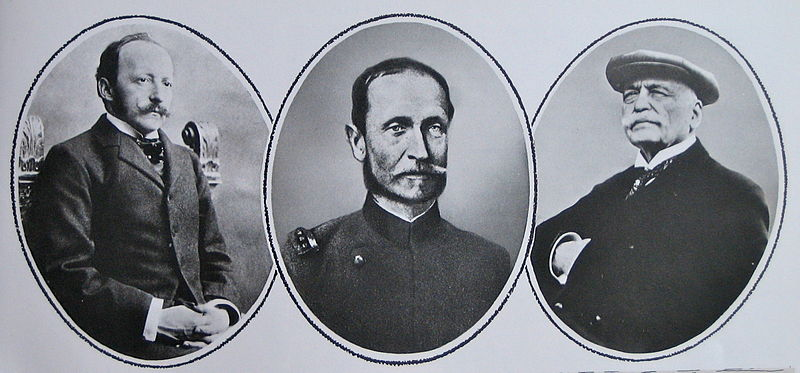
\includegraphics[width=\textwidth]{images/pfyffer.jpg}
    \caption{Max Alphons Pfyffer (in der Mitte) (unbekannt). Wikipedia. (02. Januar 2010). \newline URL: https://commons.wikimedia.org/wiki/File:C\%C3\%A9sar\_Ritz,\_Max\_Pfyffer,\_Auguste\_Escoffier.jpg [Stand 16.07.2019]}
\end{figure}

Max Alphons Pfyffer wurde am 12. Oktober 1834 in Altishofen geboren. Er war der Sohn von Heinrich Pfyffer von Altishofen. Die Familie Pfyffer von Altishofen war eine ein Patriziergeschlecht in der früheren Republik Luzern. Die Patrizierfamilien bildeten das Patriziat, welche die wichtigen Ämter in Luzern besetzten. Pfyffer von Altishofen war die mächtigste der Patrizierfamilien. Luzern war damals noch eine freie und souveräne eidgenössische Stadt und Republik. Max Alphons Pfyffer wuchs also im Adel auf.
\paragraph{}
Pfyffer war Architekt und Hotelier, er erbaute das Grand Hotel National in Luzern, welches heute noch immer in Betrieb ist. Das Hotel ist als unter Denkmalschutz, es wird als Kulturgut von nationaler Bedeutung eingestuft.
\paragraph{}
Pfyffer zeichnete auch die Pläne für die Alpenfestung Gotthard, welche auch gebaut wurde. Dadurch wurde Max Alphons Pfyffer zum Begründer des Reduit-Konzepts.
\paragraph{}
Pfyffer starb am 12. Januar 1890 55-jährig in Luzern.